\chapter{La description textuelle des données géographiques}

\label{chap:description}

% Introduction du chapitre

% Questions soulevées:
% - Pourquoi vouloir décrire le carrefour ?
% - Comment décrire une donnée géographique ?
% - Quels textes veut-on générer ? Pour quels dispositifs ?

Les descriptions textuelles et verbales font partie des outils mobilisés par les personnes concernées par la déficience visuelle pour effectuer un déplacement. Ces descriptions peuvent provenir de dispositifs de guidage, comme une application mobile, et être générées en cours de trajet et lues par synthèse vocale. Bien que les outils technologiques d'aide à la mobilité soient utilisés par une partie des personnes concernées (32\% d’après \citet{homere_2023}), les dispositifs de navigation existants ne sont pas pleinement satisfaisants à cause d’une localisation imprécise et d’informations piétonnes manquantes \citep{Guth2019}. Au niveau des carrefours notamment, ces imprécisions ne permettent pas de guider une personne de manière sécurisée, en décrivant intégralement une traversée et la qualité de son équipement. Pour un besoin spécifique et sur un itinéraire donné, un \gls{ia} peut préparer manuellement une description, dont le niveau de détails pourra par ailleurs être adapté aux besoins de la personne destinataire, et intégrer toutes les informations nécessaires en se basant sur sa connaissance du terrain. La réalisation d’une telle description est, en revanche, particulièrement chronophage, car elle est spécifique à chaque terrain étudié et chaque besoin \citep{kern2016}.

\newpar{}

Pour répondre à cette problématique de préparation de description par les \glspl{ia}, dans ce chapitre, nous allons nous intéresser à la manière de réaliser une description. Cette réalisation sera semi-automatique, en permettant notamment à l'\gls{ia} de définir la forme de la description, et s'appuiera sur des données géographiques. Nous présenterons dans un premier temps le processus général, fortement basé sur les capacités d’un \gls{sig} et nécessitant par conséquent des connaissances spécifiques, puis nous montrerons son application à différentes typologies de descriptions qui peuvent aller au-delà du texte linéaire.

\section{Des données géographiques au texte}

\label{sec:description_geodata_to_text}

Nous avons vu dans le chapitre \ref{chap:modelisation} qu’il pouvait exister des données suffisamment complètes pour proposer une modélisation du carrefour. Cette modélisation peut avoir des applications multiples (voir chapitre \ref{chap:implementation}) dont la génération d’une description textuelle de celui-ci en suivant une approche données vers texte \citep{reiter-2007-architecture}. Cette approche a notamment été suivie par \citet{Guth2019} et \citet{balata2018} pour produire des descriptions de carrefours et de leurs traversées, mais en utilisant des données conçues à cet effet et non des données issues d’une base de données publique. Par ailleurs, les descriptions proposées sont figées, adaptées à un contexte unique qui ne correspond pas forcément à la variété des besoins exprimés par les \glspl{ia} et les personnes concernées. Au-delà du carrefour, des besoins spécifiques peuvent impliquer la modulation du texte (vocabulaire, verbosité), mais également l’intégration de données nouvelles pour décrire des éléments extérieurs à la voirie (par exemple, les arrêts de bus). Ainsi, nous souhaitons proposer un outil flexible qui permettrait à l’instructeur de concevoir une description selon les besoins exprimés et de générer le texte correspondant sur les différents territoires étudiés lors des séances de locomotion. L’ajout de données arbitraires amène à généraliser le problème à la création d’un texte depuis toute donnée géographique.

\newpar{}

Plusieurs problématiques émergent cependant de cette possibilité: au sujet des carrefours, les chapitres \ref{chap:modelisation} et \ref{chap:evaluation} montrent que les données ou les résultats des traitements algorithmiques sur celles-ci sont parfois incomplets ou incorrects et peuvent nécessiter une correction. Par ailleurs, toute donnée n’est pas nécessairement adaptée à une verbalisation et peut nécessiter un traitement en amont pour la textualiser, à l’instar des traitements réalisés sur une donnée pour la cartographier \citep{mackaness2002}. Ces traitements sont généralement réalisés au sein d’un \gls{sig} par un cartographe ou un géomaticien. Les \glspl{ia} comme les adaptateurs-transcripteurs n’ont généralement pas les connaissances pour manipuler ces outils. Pour répondre à ces problématiques d'adaptation de données, nous proposons d’ajouter le géomaticien comme intermédiaire supplémentaire à la chaîne de génération de description. Ce dernier sera ainsi l’utilisateur principal de l’outil proposé et pourra intégrer les besoins des différentes parties au sein d’une chaîne de traitements de données géographiques permettant de générer du texte.

\subsection{Définition de la description}

Pour lire des documents textuels virtuels, les personnes déficientes visuelles utilisent généralement un lecteur d’écran, un logiciel qui retranscrit par synthèse vocale ce qui est affiché sur l’écran du terminal. Une particularité des lecteurs d’écran est qu’ils ne font pas une simple retranscription texte vers voix, mais qu’ils retranscrivent aussi la structure du document lu. Cela signifie qu’en parcourant le document, la personne sera informée des titres, des paragraphes, des listes, etc. La lecture est par ailleurs interactive: il est possible de sauter un paragraphe, de revenir au précédent, ou encore de parcourir un à un les éléments d’une liste.

\newpar{}

Dans la suite de ce chapitre, une description sera définie par un texte possiblement augmenté, c’est-à-dire un texte dont les éléments sont annotés pour enrichir son contenu \citep{oren2006semantic} (voir figure \ref{fig:desc_ex_texte_annoté}). Ces annotations permettent notamment la réalisation d’un document structuré, mais aussi d’organiser les textes entre eux.

\begin{figure}[ht]
    \centering
    \begin{subfigure}{0.49\textwidth}
        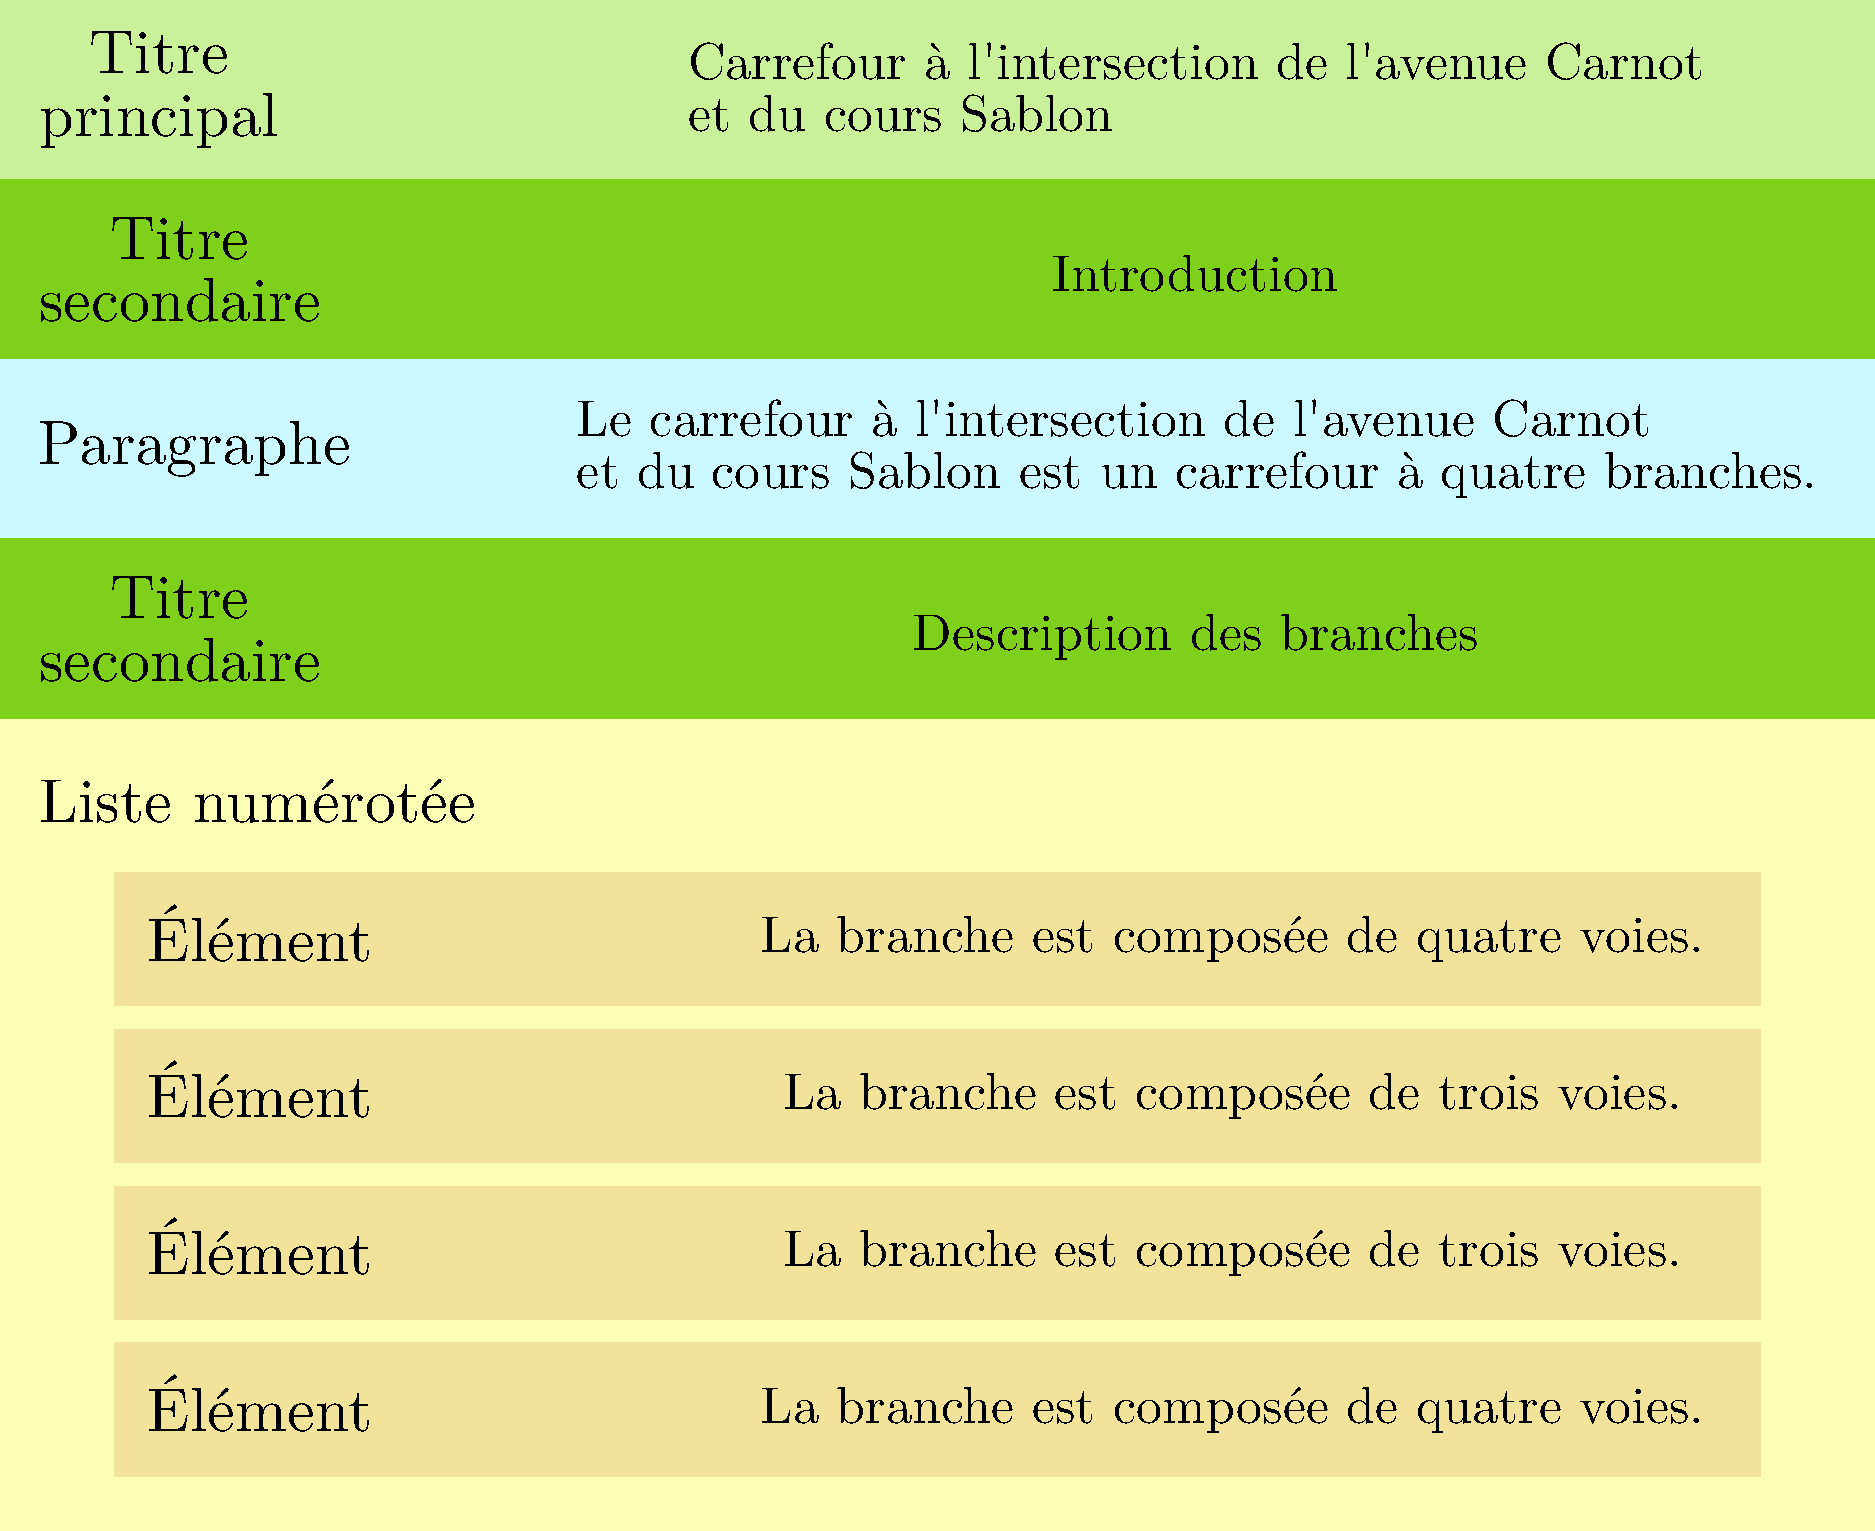
\includegraphics[width=0.95\textwidth]{images/description/exemple_texte_augmente_1.pdf}
        \label{fig:desc_ex_texte_annoté_1}
        \caption{Texte annoté.}
    \end{subfigure}
    \begin{subfigure}{0.49\textwidth}
        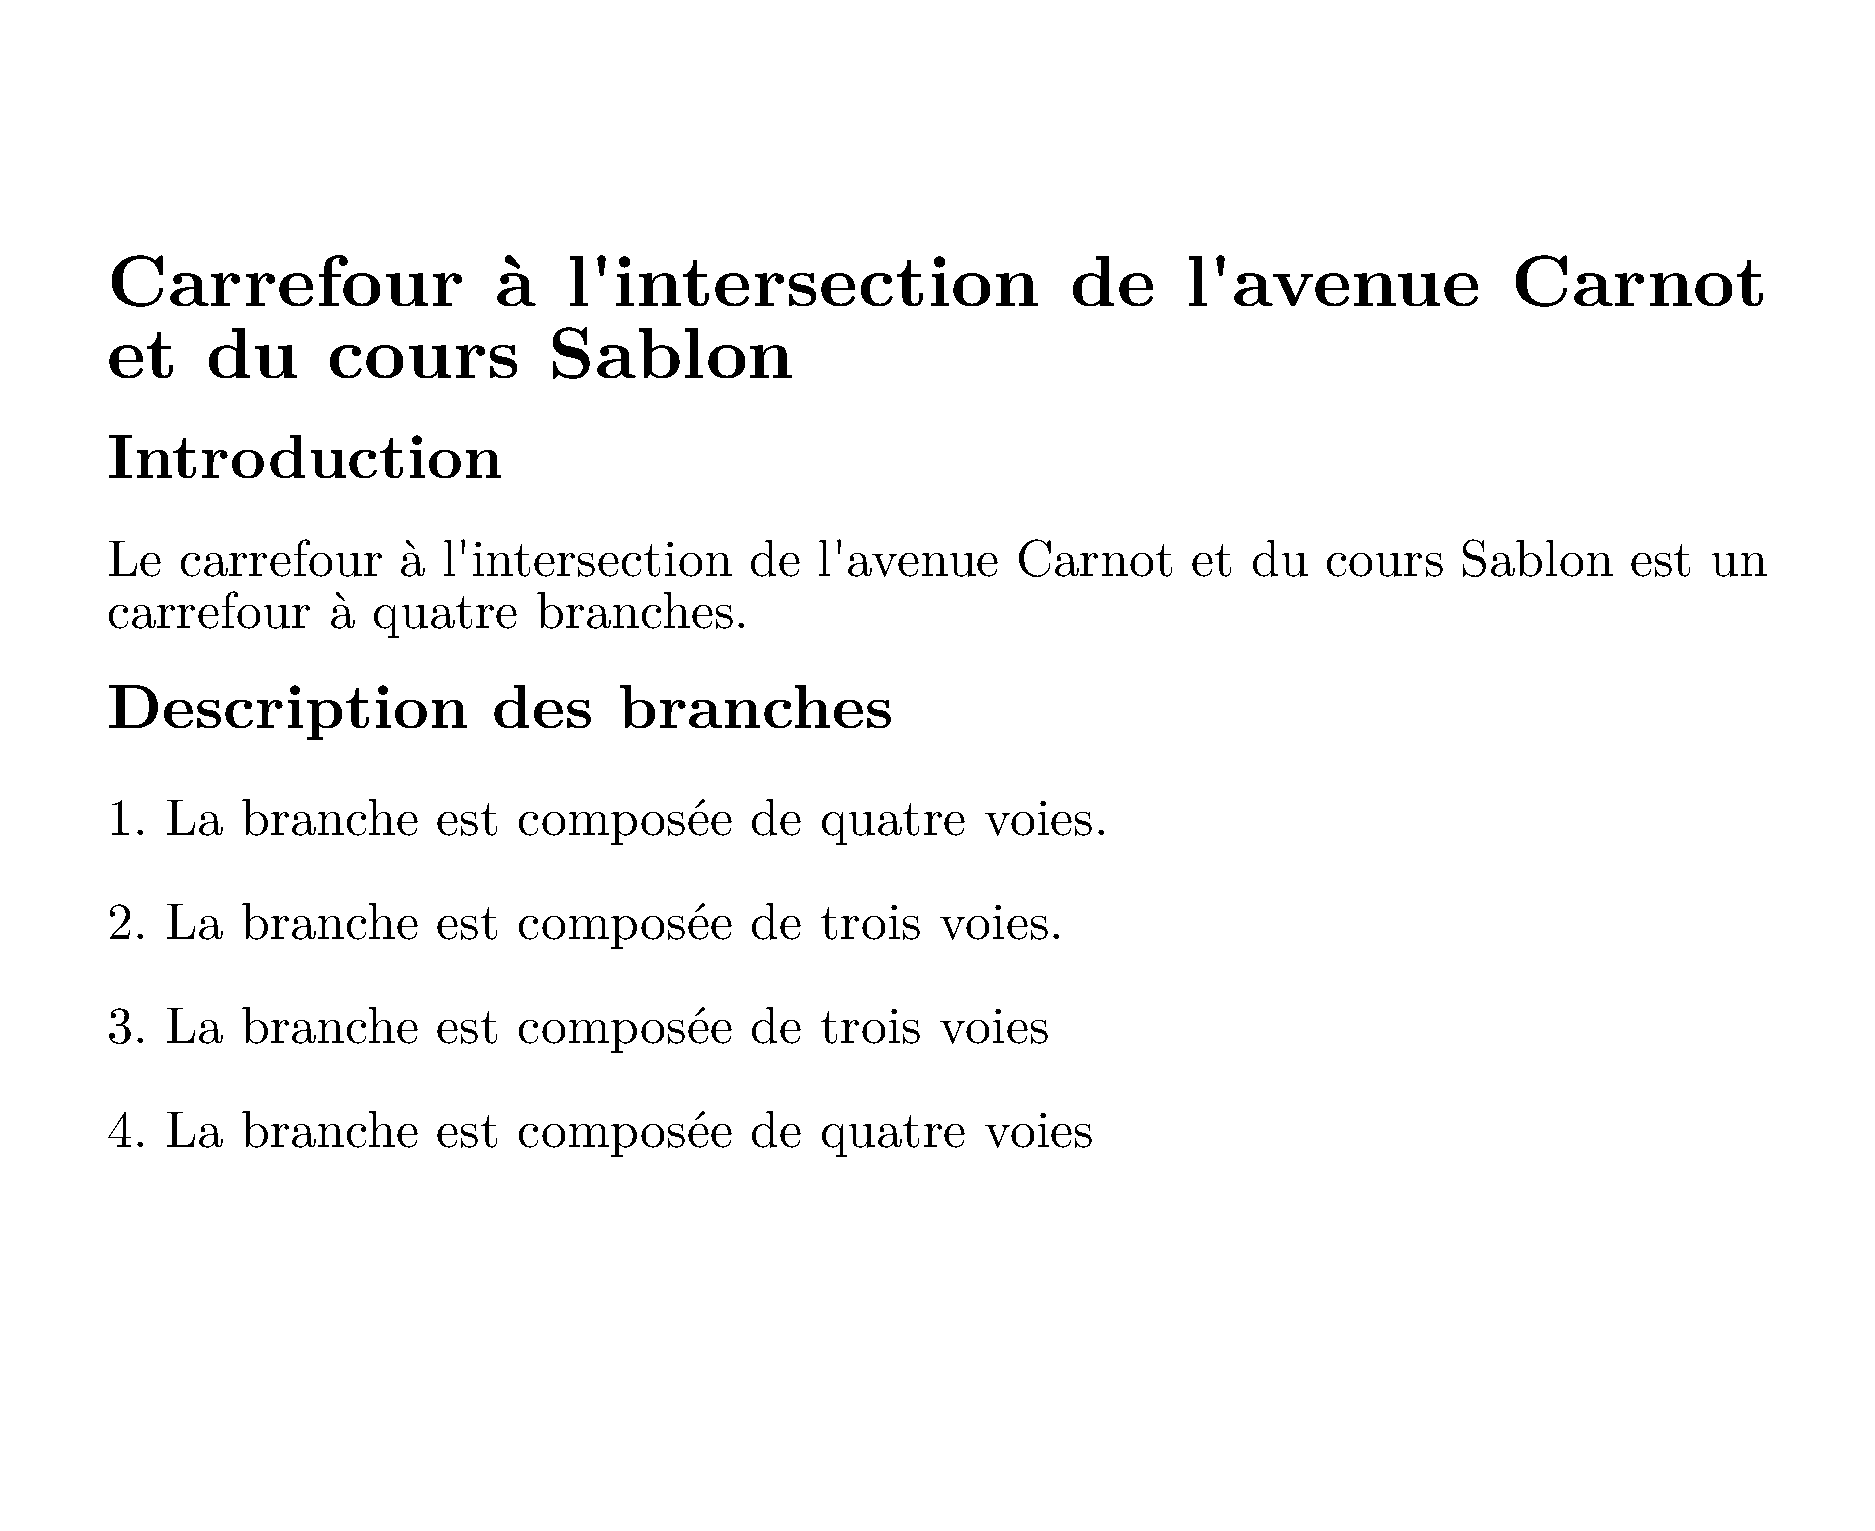
\includegraphics[width=0.95\textwidth]{images/description/exemple_texte_augmente_2.pdf}
        \label{fig:desc_ex_texte_annoté_2}
        \caption{Exemple de rendu du texte annoté.}
    \end{subfigure}
    \caption[Exemple de texte annoté.]{Exemple de texte dont les annotations définissent la structure du document.}
    \label{fig:desc_ex_texte_annoté}
\end{figure}

\subsection{Spécification du système de conception de description}

Un \gls{sig} est un système informatique permettant l’acquisition, le stockage, l’interrogation, le traitement, l’analyse, et la visualisation de données géographiques \citep{AschanLeygonie2019}. Il peut s’agir d’un logiciel de bureau utilisable au travers d’une interface graphique ou d’un système de gestion de bases de données spatiales. Le modèle de représentation le plus courant au sein d'un \gls{sig} consiste en un empilement de couches thématiques: chaque couche étant un fichier indépendant avec ses propres attributs et métadonnées (projection, sémantique, géométrie). On distingue en général les couches de type raster (image multispectrale dont chaque pixel a une valeur) des couches de type vecteur (donnée tabulaire dont un ou plusieurs champs peuvent contenir une géométrie), ces dernières ayant un fonctionnement proche des tables telles qu’elles existent dans les \gls{sgbdr}. 

\newpar{}

Un des intérêts des \gls{sig} concerne la possibilité d’y réaliser des chaînes de traitements, c’est-à-dire une succession de traitements appliqués à un ensemble de données en entrées pour obtenir un nouvel ensemble de données en sorties. Cela peut inclure entre autres des sélections basées sur la sémantique ou la géométrie, des jointures entre couches et des modifications ou des créations de champs attributaires ou géométriques. Ces chaînes permettent de généraliser un traitement complexe pour l’appliquer sur plusieurs ensembles de données et sur plusieurs territoires. À l’instar des traitements qu’elles embarquent, elles peuvent également être paramétriques afin de piloter leur exécution si nécessaire. Des outils se reposant sur ce système de chaînes de traitement \gls{sig} ont déjà été proposés par la littérature, par exemple pour réaliser des « cartes à la carte » \citep{bucher2007} ou généraliser des données géographiques \citep{lee2001,petzold2006}.

\newpar{}

Le cadre de conception de description que nous proposons se repose sur une chaîne similaire à celle que l’on pourrait mobiliser pour générer une carte. En effet, la réalisation d’une carte repose sur trois grandes étapes: la spécification du style, où l’on détermine la forme que l’on souhaite obtenir, le rendu, où l’on mobilise des outils pour traiter les données, et la visualisation, où l’on exécute la chaîne pour obtenir le résultat final \cite{christophe2016}. En effectuant un parallèle:

\begin{itemize}
    \item La spécification du style correspond à la conception d'un canevas modulaire. On entend par canevas modulaire la définition des textes finaux que l'on souhaite obtenir et des formes textuelles à appliquer à chaque donnée représentée. Plus de détails sur cette étape sont donnés en partie \ref{sec:conception_canevas}.
    \item Le rendu correspond aux traitements qui seront appliqués sur les données pour les adapter au contexte et permettre leur textualisation. Plus de détails sur cette étape sont donnés en partie \ref{sec:conception_chaine_sig}.
    \item La visualisation correspond à l’exécution de la chaîne de traitements par l'utilisateur final, en agissant sur les éventuels paramètres exposés par la chaîne de traitement,  pour obtenir le résultat final.
\end{itemize}

\newpar{}

Dans notre cas, plusieurs acteurs seront mobilisés à chaque étape. En effet, on considère que l’\gls{ia} se repose sur un géomaticien pour la conception technique de la chaîne de traitement. En revanche, il conserve un rôle de concepteur: il doit ainsi avoir une idée précise du résultat souhaité pour en permettre l’implémentation. Ces différentes étapes sont détaillées dans les parties suivantes.

\subsubsection{Conception d'un canevas modulaire}

\label{sec:conception_canevas}

Cette première étape consiste à définir exactement les besoins, qui vont notamment s’exprimer par la sortie souhaitée. Pour cela, l’\gls{ia} va concevoir les formes de description finales: quels seront les textes et leurs éventuelles variations, quels seront leur agencement et leur mise en forme (voir parties \ref{sec:description_textuelle}, \ref{sec:description_carte} et \ref{sec:description_graphe}).

\newpar{}

Avec cette vision finale de la description, l’instructeur peut déterminer la forme des données nécessaires pour réaliser la description. Il ne s’agit pas ici de déterminer les données disponibles (qui seront acquises et traitées par un géomaticien comme décrit en partie \ref{sec:conception_chaine_sig}), mais d’estimer les données thématiques et les attributs nécessaires afin, pour chacune, de définir un patron, c’est-à-dire un algorithme produisant un texte qui pourra varier selon les attributs des données. Par ailleurs, il est possible de définir plusieurs patrons pour une donnée, chacun correspondant à un usage (par exemple un patron synthétique et un patron détaillé). Chaque patron peut être complété de métadonnées permettant de le caractériser et dont le choix est à la discrétion de l’instructeur.

\newpar{}

On parle de canevas modulaire, car la forme finale de la description n’est pas nécessairement figée et peut varier selon des paramètres définis à la conception. Il peut s’agir lors de l’assemblage du texte final de la sélection de patrons spécifiques et de leur ordonnancement, ou de variations sur le vocabulaire.

\newpar{}

Un exemple de conception de canevas est illustré en figure \ref{fig:desc_canevas_modulaire} pour décrire l'accessibilité des boulangeries de Clermont-Ferrand. 

\begin{figure}[ht]
    \centering
    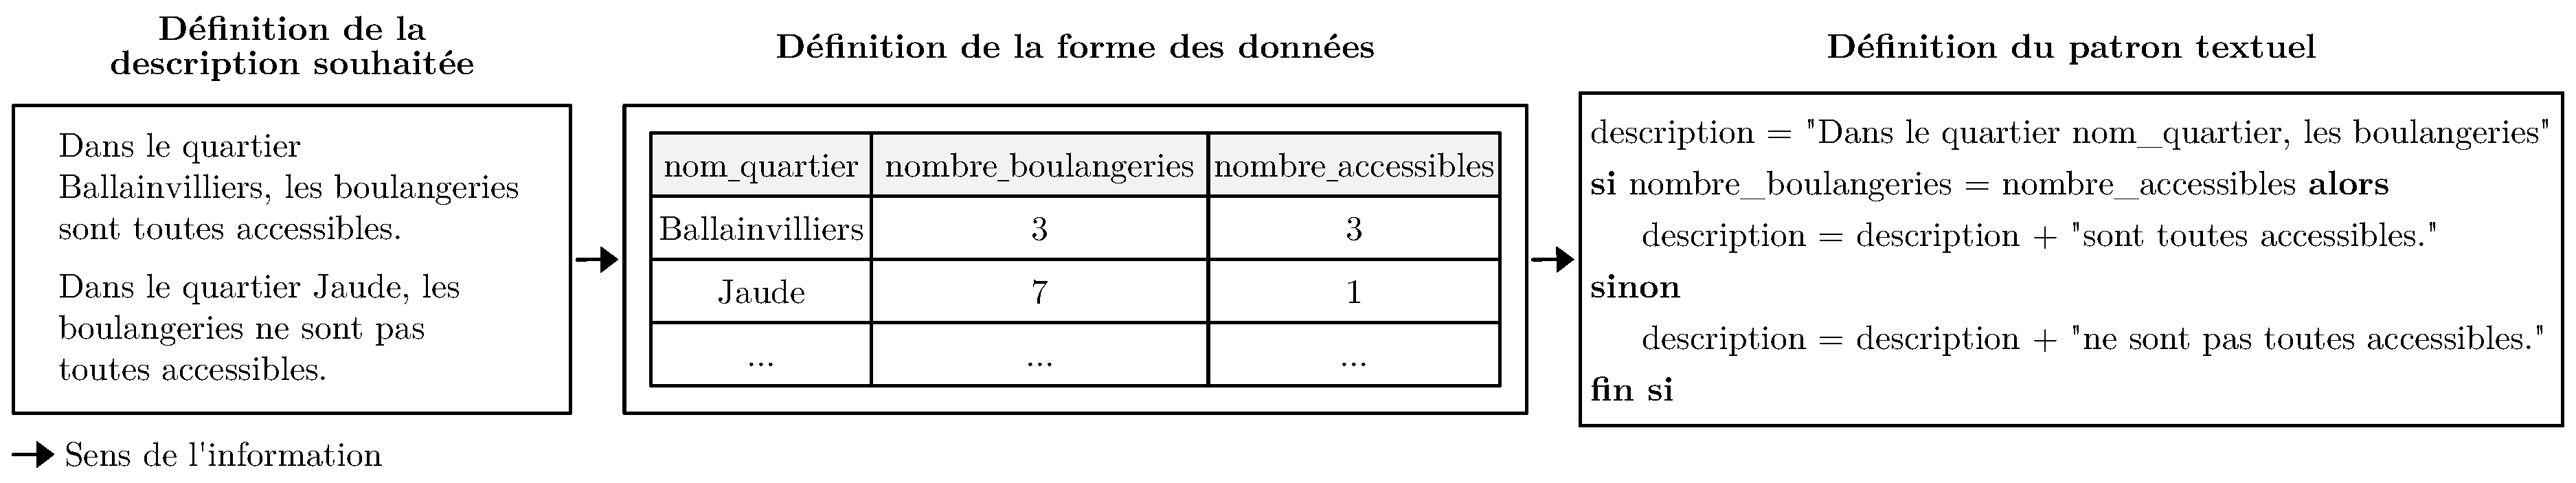
\includegraphics[width=\textwidth]{images/description/exemple_canevas.pdf}
    \caption[Exemple de canevas de description]{Cet exemple illustre la conception d'un canevas pour générer un résumé par quartier de l'accessibilité des boulangeries.}
    \label{fig:desc_canevas_modulaire}
\end{figure}

Il se découpe en trois étapes:

\begin{enumerate}
    \item \textbf{Définition de la description souhaitée:} L'\gls{ia} définit le texte qu'il souhaite obtenir en fin de chaîne.
    \item \textbf{Définition de la forme des données:} À partir du texte défini à l'étape précédente, l'\gls{ia} détermine quelles données sont nécessaires pour le générer. Dans cet exemple, on a besoin d'une table de données qui définit pour chaque quartier ($nom\_quartier$) le nombre de boulangeries qu'il contient ($nombre\_boulangeries$) et le nombre de boulangeries accessibles ($nombre\_accessibles$). 
    \item \textbf{Définition du patron textuel:} Enfin, l'\gls{ia} définit le patron à associer à la table de données précédente. Le patron correspond à un texte conditionnel qui varie en fonction des données. Dans cet exemple, le nombre de boulangeries accessibles est comparé au nombre total de boulangeries pour déterminer si toutes les boulangeries du quartier sont accessibles. Le texte final est alors généré en fonction de cette comparaison. 
\end{enumerate}

\subsubsection{Conception de la chaîne de traitement \gls{sig}}

\label{sec:conception_chaine_sig}

Après la définition du besoin par l’\gls{ia}, le géomaticien a en charge l’implémentation de la chaîne de traitements au sein d’un \gls{sig}. Pour cela, il doit tout d’abord identifier et évaluer les sources de données disponibles au regard du besoin. L’évaluation comprend ici la précision des données, qui peut être à la fois la précision métrique, mais aussi le niveau de détails (pour un trottoir par exemple, a-t-on besoin de lignes ou de polygones ?) ou encore la couverture géographique (est-ce que la description doit pouvoir s’appliquer partout ou sur un territoire donné ?).

\newpar{}

Une fois les données identifiées, il peut réaliser la chaîne de traitements \gls{sig} qui s’articule autour des trois étapes suivantes:

\begin{enumerate}
    \item \textbf{Transformation des données pour les adapter au contexte}\\
            \textbf{Entrée}:\\
            \hspace*{1cm}Données géographiques\\
            \textbf{Sortie}:\\
            \hspace*{1cm}Données géographiques\\
            En ayant maintenant les données à sa disposition, le géomaticien peut utiliser les outils du \gls{sig} pour réaliser des traitements sur celles-ci. À l’instar des traitements réalisés pour faire une carte (généralisation géométrique, conception de nouveaux indicateurs) il s’agit ici d’adapter les données à l’usage, ici la réalisation du texte déterminé par les patrons. Cela peut signifier calculer de nouveaux champs, résumer une donnée, réaliser des jointures, etc. Les traitements pourront différer d’une donnée à l’autre et d’une description à l’autre. Les nouvelles tables obtenues doivent correspondre à celles définies par l’\gls{ia} à l’étape de conception du canevas.
    \item \textbf{Implémentation des patrons conçus par l’\gls{ia}}\\
        \textbf{Entrée}:\\ 
        \hspace*{1cm}Données géographiques\\
        \textbf{Sortie}:\\
        \hspace*{1cm}Données géographiques décrites\\
        Pour chaque couche en entrée, le géomaticien implémente les patrons conçus par l’instructeur dans le langage de programmation permis par le \gls{sig}. Il définit également l’ensemble des métadonnées associées aux couches pour permettre leur sélection dans l’étape d’assemblage. Cette étape permet de générer un texte correspondant au patron pour chaque entité de la couche un texte.
    \newpage
    \item \textbf{Assemblage des textes en description}\\
        \textbf{Entrées}:\\
        \hspace*{1cm}Données géographiques décrites\\
        \hspace*{1cm}Plan de description \\
        \textbf{Sortie}:\\
        \hspace*{1cm}Description\\
        Cette étape correspond à l’assemblage qui va permettre d'obtenir la description finale en accord avec le canevas établi par l’\gls{ia}. Le plan de description en entrée permet de sélectionner et d’agencer les couches décrites au sein de la description. C'est cette étape d'assemblage qui assure également l'augmentation du texte final. Ainsi, en fonction du type de description à produire, le fonctionnement de cette étape peut varier (voir partie \ref{sec:description_cas_utilisation}).
\end{enumerate}

Chaque étape peut être implémentée dans le \gls{sig} sous la forme d’un algorithme pouvant être exécuté par l'utilisateur final, l'\gls{ia}. Les paramètres de ces algorithmes peuvent être exposés pour permettre à l’utilisateur de piloter l’exécution de la chaîne de traitement.

\newpar{}

Le processus illustré en figure \ref{fig:desc_chaine_sig} poursuit l'exemple de la figure \ref{fig:desc_canevas_modulaire} en présentant une implémentation possible de la chaîne de traitement pour générer un résumé par quartier de l'accessibilité des boulangeries. Les données utilisées pour l'exemple sont fictives. 

\begin{figure}[ht]
    \centering
    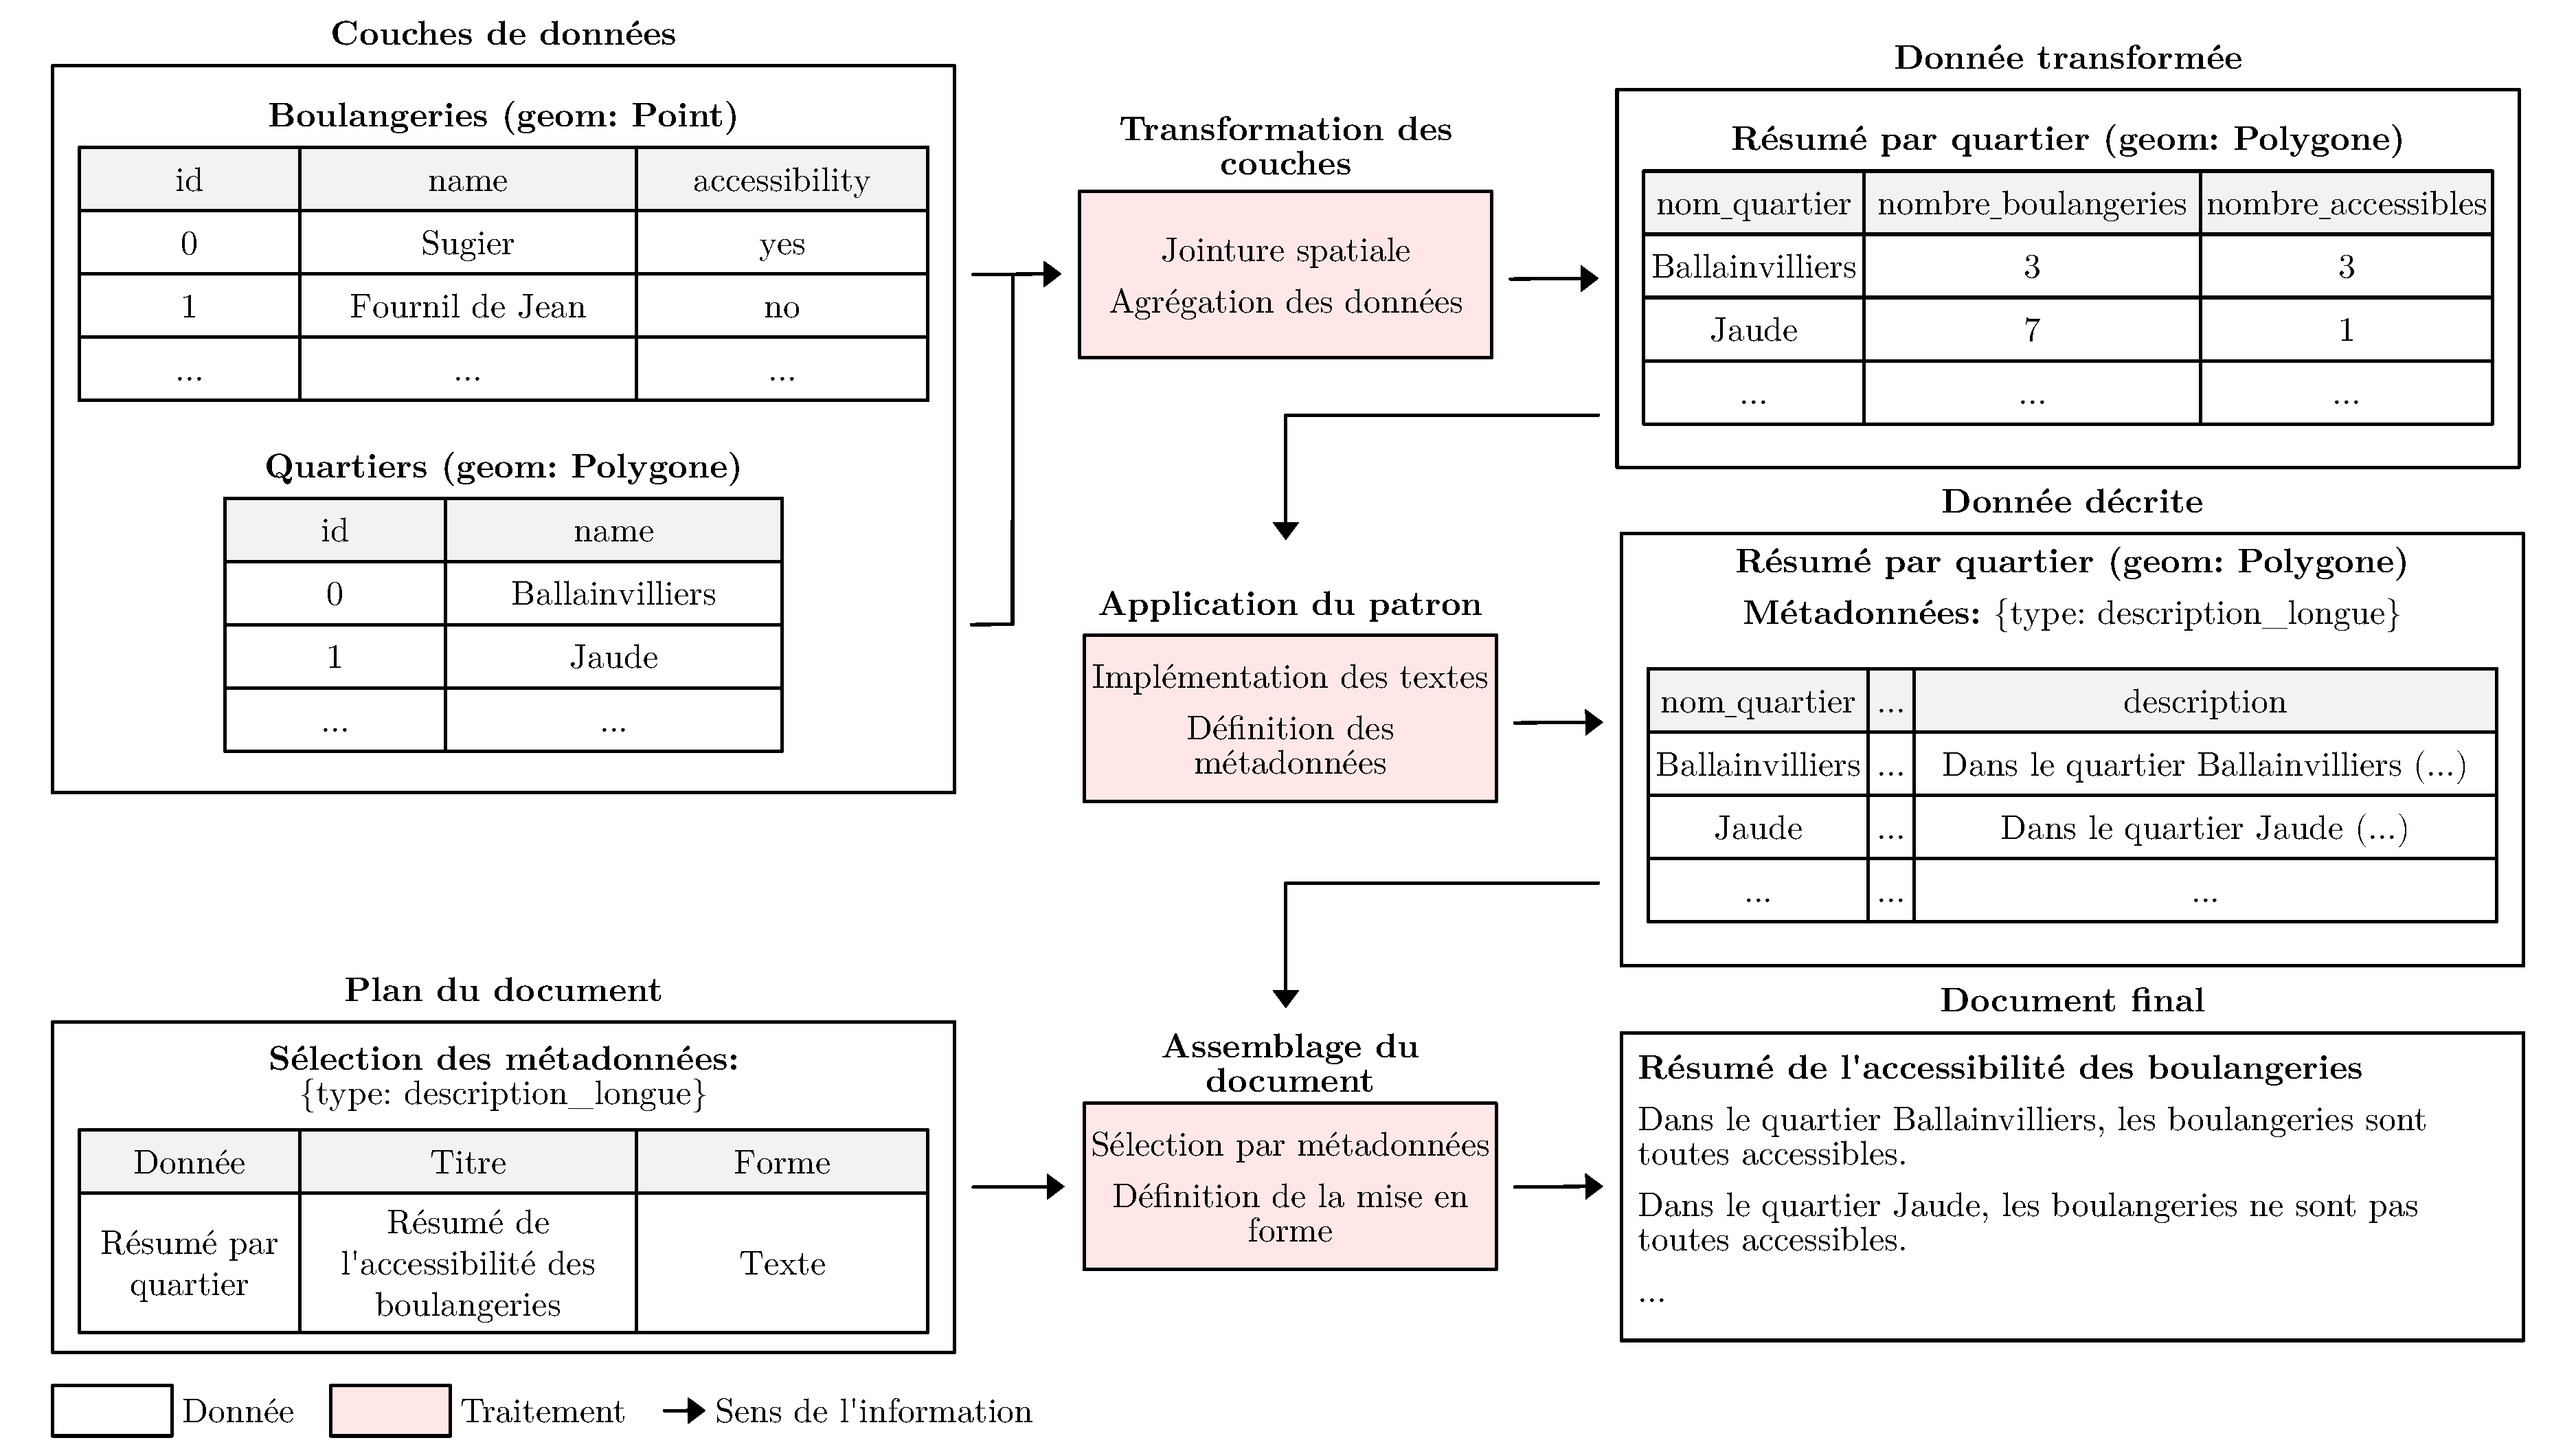
\includegraphics[width=\textwidth]{images/description/exemple_chaine.pdf}
    \caption[Chaîne de traitement de réalisation de description]{La chaîne de traitement produite par le géomaticien pour générer l'exemple des boulangeries.}
    \label{fig:desc_chaine_sig}
\end{figure}

Le processus reprend les trois étapes précédemment décrites:

\begin{enumerate}
    \item \textbf{Transformation des données:} La première brique implémentée par le géomaticien réalise un traitement de jointure spatiale entre les boulangeries (représentées sous forme de points) et les quartiers (délimités par des polygones) pour obtenir la table définie par l'\gls{ia} en figure \ref{fig:desc_canevas_modulaire} qui recense par quartier le nombre total de boulangeries et le nombre de boulangeries accessibles.
    \item \textbf{Application du patron:} En figure \ref{fig:desc_canevas_modulaire}, l'\gls{ia} avait défini un patron à appliquer à la table du résumé des boulangeries par quartier. Dans cette étape, le géomaticien implémente ce patron à l'aide d'un langage de programmation dans le \gls{sig}.L'exécution de cette brique permet d'obtenir, pour chaque entité de la table, le texte qui résume l'accessibilité des boulangeries dans le quartier. Les métadonnées, utilisées pour sélectionner les couches à assembler, sont en réalité facultatives dans cet exemple comme il n'y a qu'une seule couche. Il aurait été possible de définir deux types de description, par exemple $description\_courte$ et $description\_longue$ pour permettre à l'utilisateur final de choisir le niveau de détail de la description.
    \item \textbf{Assemblage du document:} En prenant en entrée la couche dont les entités ont été décrites à l'étape précédente, et un plan de description permettant d'ordonner les couches décrites (même s'il n'y en a qu'une seule dans cet exemple), cette brique permet d'assembler les descriptions au sein d'une description augmentée structurée. On obtient alors un document analogue au texte défini par l'\gls{ia} en figure \ref{fig:desc_canevas_modulaire}.
\end{enumerate}

\subsubsection{Point de vue adopté par le texte}

% 1. Définition
On appelle description exocentrée une description dont la position des éléments spatiaux est décrite de manière externe et non de manière relative à un point interne à l'espace décrit. De ce point de vue, la lecture d'une description exocentrée est donc analogue à la lecture d'une carte topographique qui adopte généralement un point de vue également exocentré. Cependant, comme présenté dans la partie \ref{sec:description_geodata_to_text}, une description exocentrée ne décrit pas nécessairement des données brutes. Un traitement adapté au texte voulu peut être réalisé sur celles-ci pour intégrer du contexte spatial. Ainsi, il est possible dans une description exocentrée de décrire une relation spatiale (<<~la boulangerie est dans un quartier~>>) ou une orientation relative aux points cardinaux (<<~au sud du carrefour (...)~>>).

\newpar{}

Une description égocentrée est à l'inverse de la description exocentrée une description localisée, relative à un point interne à l'espace décrit. Le sujet est placé au sein de l'environnement, et le texte peut alors mobiliser des prépositions spatiales telles que <<~en face~>>, <<~à droite~>>...

\section{Réaliser différents types de descriptions}

\label{sec:description_cas_utilisation}

Le cadre présenté en partie \ref{sec:description_geodata_to_text} permet de générer du texte brut ou augmenté depuis toute donnée géographique. Si les étapes de traitement des données géographiques et d'applications des patrons sont standards peu importe le type de sortie souhaitée, nous avons évoqué que l'étape d'assemblage est à adapter par le géomaticien selon le type de description à produire. Dans cette partie, nous allons illustrer comment le cadre présenté et cette dernière étape d'assemblage peuvent être adaptés pour produire différents types de descriptions augmentées.

\subsection{La réalisation d'une description linéaire}

\label{sec:description_textuelle}

La description linéaire est la forme la plus simple de description. Elle consiste en un texte qui décrit les éléments de manière séquentielle. Cette description peut être structurée pour en faciliter la navigation à l'aide d'un lecteur d'écran. Il s'agit du type de description illustré par les figures \ref{fig:desc_ex_texte_annoté}, \ref{fig:desc_canevas_modulaire}, et \ref{fig:desc_chaine_sig}. La sortie pourrait être par exemple un document HTML, les annotations de structure évoquées en figure \ref{fig:desc_ex_texte_annoté} pouvant être transformées en balises HTML entourant le texte annoté par la brique d'assemblage (voir figure \ref{fig:desc_ex_desc_lineaire}).

\begin{figure}[ht]
    \centering
    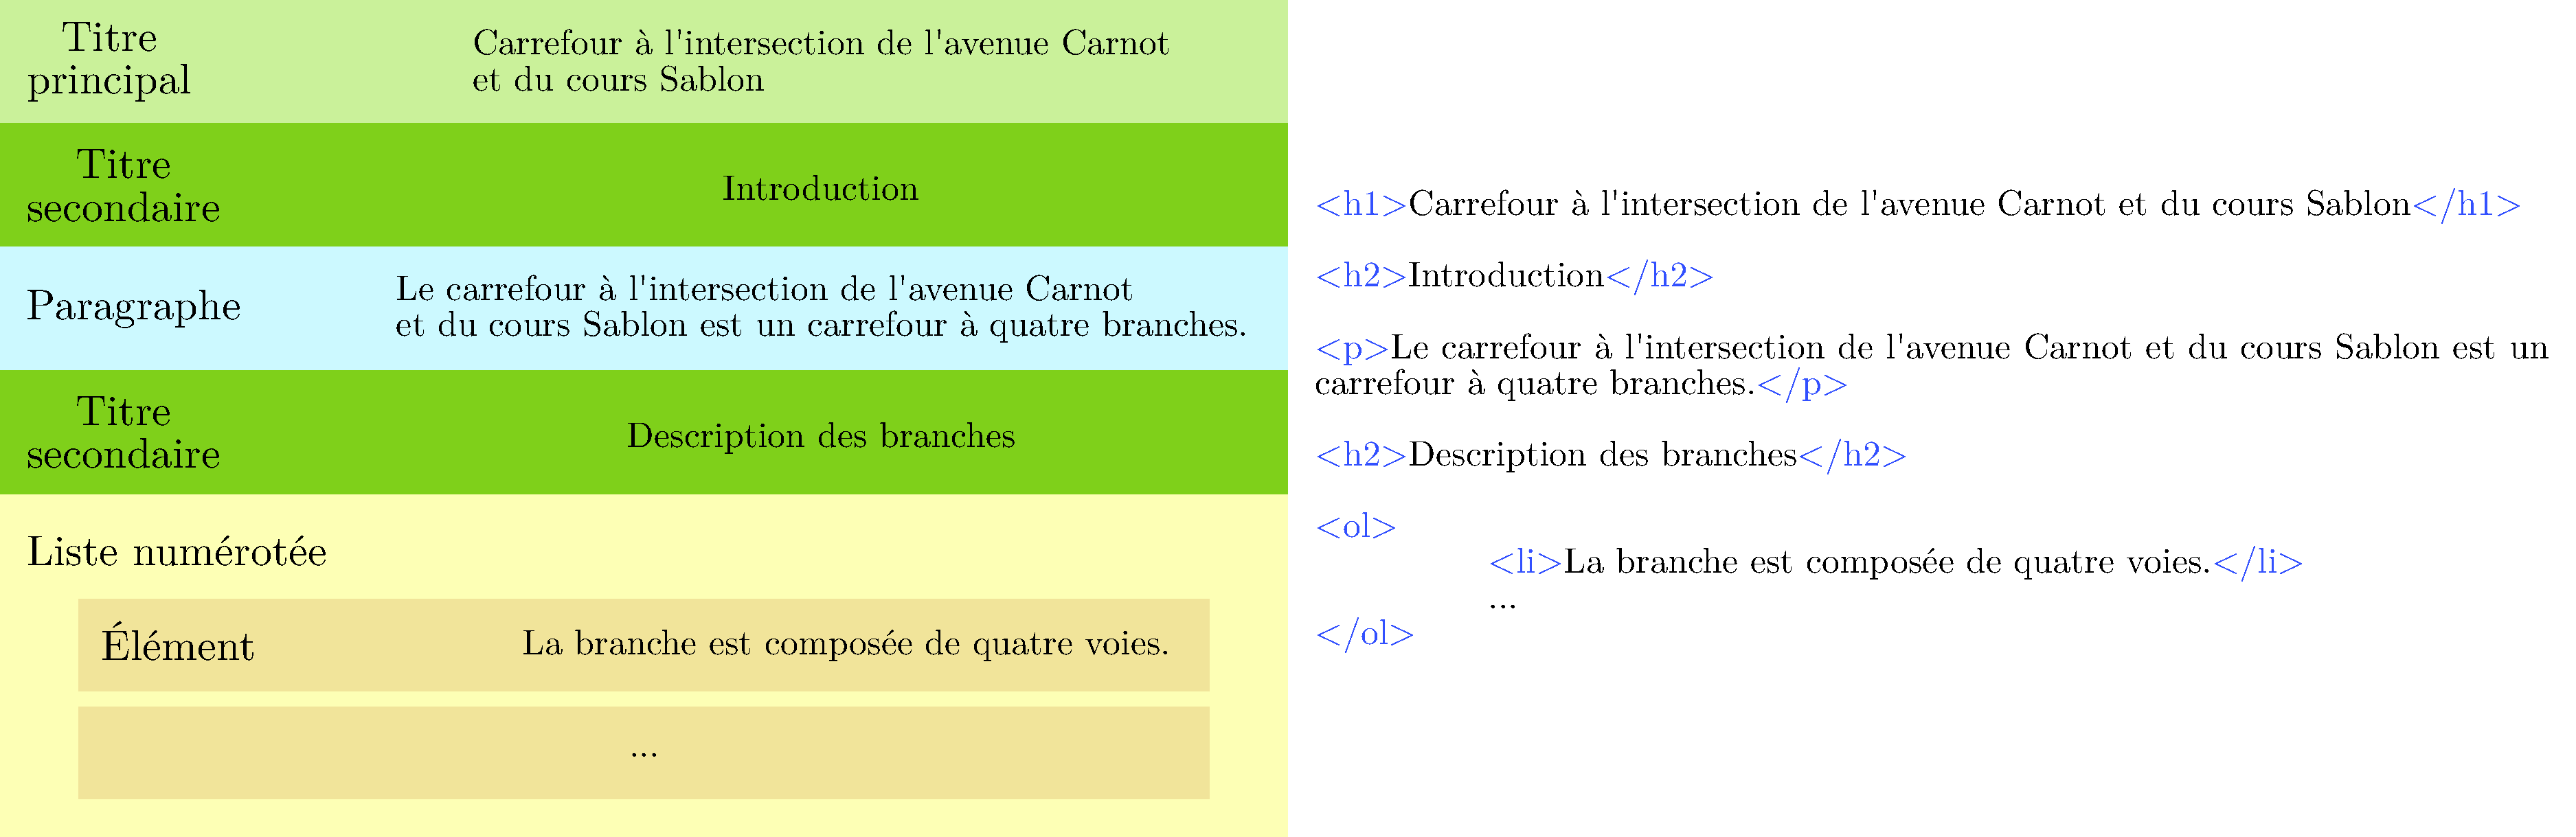
\includegraphics[width=\textwidth]{images/description/exemple_desc_lineaire.pdf
    }
    \caption[Exemple de description linéaire.]{Exemple de description linéaire: le texte annoté en sections est transformé en HTML par la brique d'assemblage.}
    \label{fig:desc_ex_desc_lineaire}
\end{figure}

\subsection{La réalisation d'une description spatialisée}

\label{sec:description_carte}

Une description, si elle conserve des attributs géographiques, peut également être intégrée au sein d'une carte interactive. Si toute carte dématérialisée permet d'embarquer du texte au sein des objets qu'elle représente (généralement accessible par une infobulle), des dispositifs physiques tels que \gls{deri} \citep{Brock2012} ou TouchIt3D \citep{barvir2021} permettent de déclencher un son lors de l'appui sur un interacteur. Comme évoqué précédemment, lors de la réalisation du canevas modulaire, on associe un texte à chaque entité décrite. Lors de cette étape, il s'agit d'un attribut supplémentaire contenant le texte qui est ajouté à la donnée originale. Ainsi, la dimension géographique n'est pas perdue, et il est alors possible d'intégrer ces entités non au sein d'un document textuel, mais d'une carte qui permet d'accéder à la description de chaque entité (voir figure \ref{fig:desc_ex_desc_spatialisee}).

\begin{figure}[ht]
    \centering
    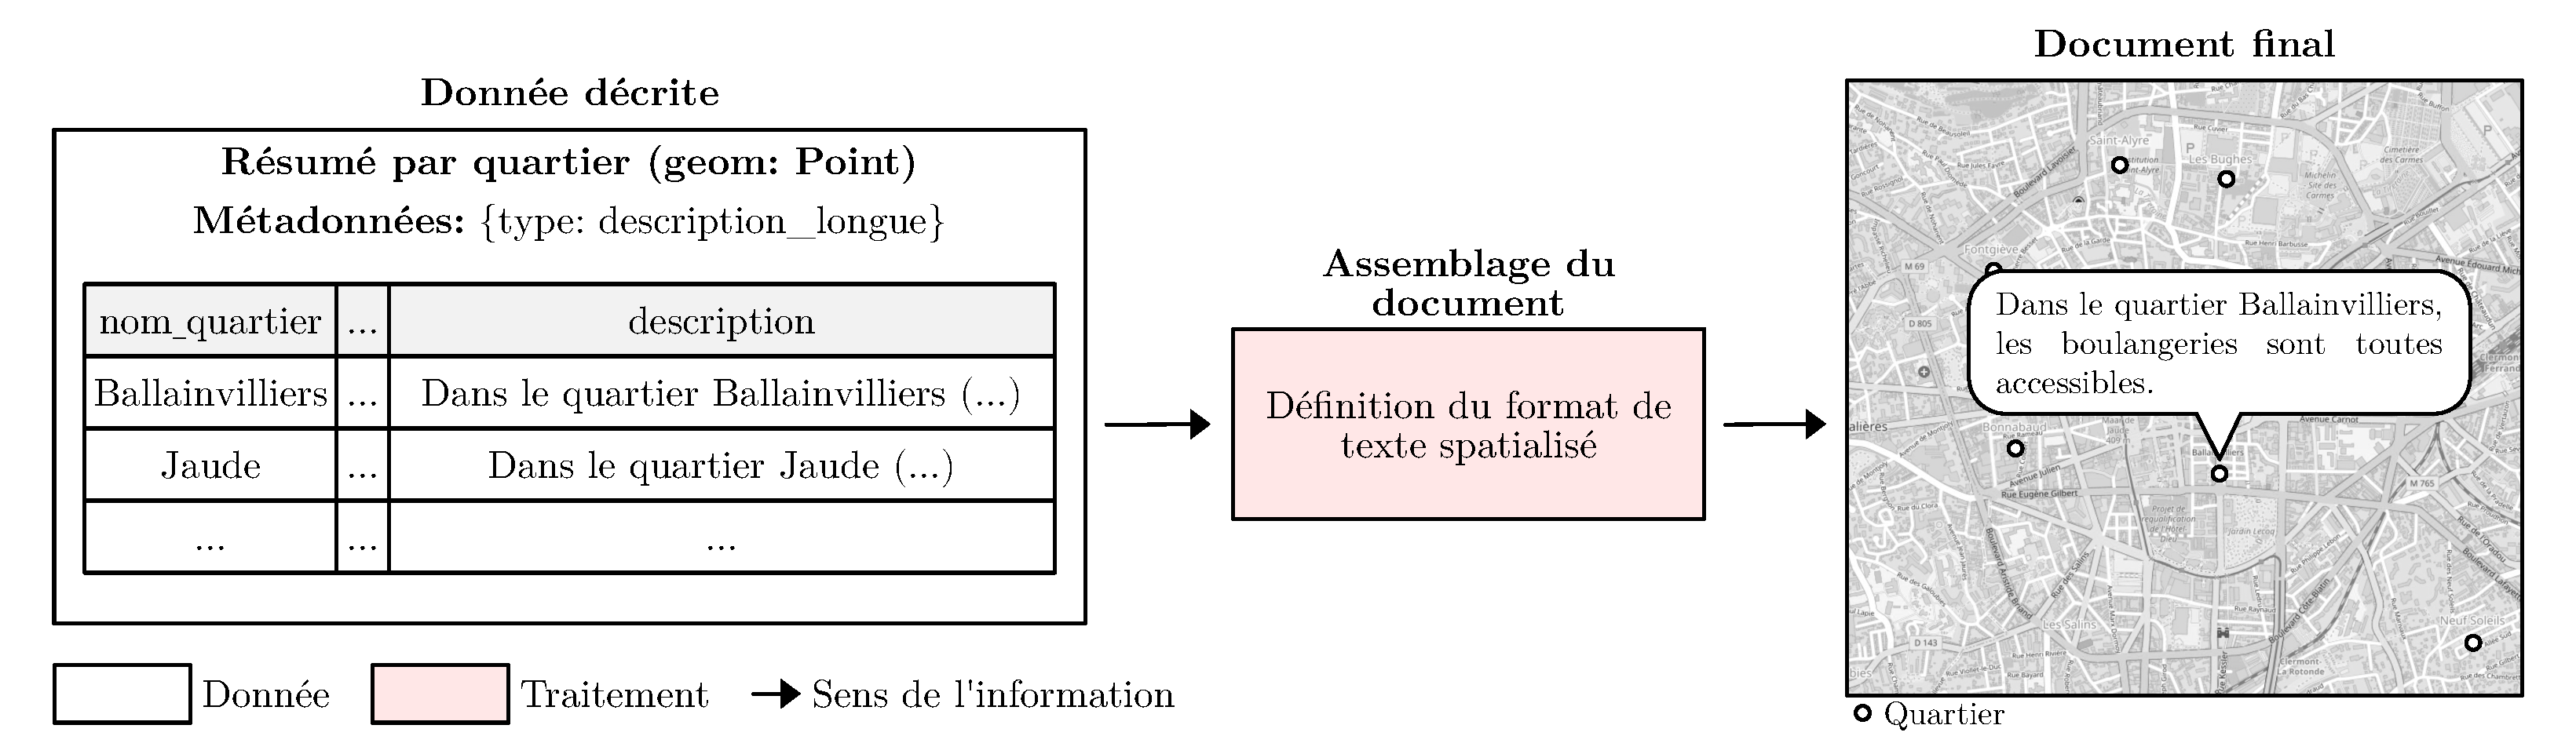
\includegraphics[width=\textwidth]{images/description/exemple_desc_spatialise.pdf
    }
    \caption[Exemple de description spatialisée.]{Exemple de description intégrée à une carte: la brique d'assemblage permet la production d'un texte formaté pour une représentation spatialisée comme par exemple le format défini par \gls{deri} (voir partie \ref{sec:experimentation_generer_deri}).}
    \label{fig:desc_ex_desc_spatialisee}
\end{figure}

\subsection{La réalisation d'une description sous forme de graphe}

\label{sec:description_graphe}

Le cadre défini dans la partie \ref{sec:description_geodata_to_text} présente une description comme un ensemble de textes augmentés pouvant embarquer des informations supplémentaires pouvant permettre une mise en forme élaborée de la description finale. Une des mises en forme possible consiste en la création d'un graphe de textes. En définissant pour chaque entité un ensemble de voisins pour former un graphe, puis en décrivant chaque entité, il devient possible de représenter la topologie d'un environnement sous forme de textes. La figure \ref{fig:desc_graphe_texte} illustre un exemple de résultat qui pourrait être issu de la description d'un graphe représentant une rue et ses commerces. Des supports permettant la navigation dans ce type de graphe sont présentés en parties \ref{sec:experimentation_poc2} et \ref{sec:experimentation_le_carrefour_dont_vous_etes_le_heros}.

\begin{figure}[ht]
    \centering
    \resizebox{15cm}{!}{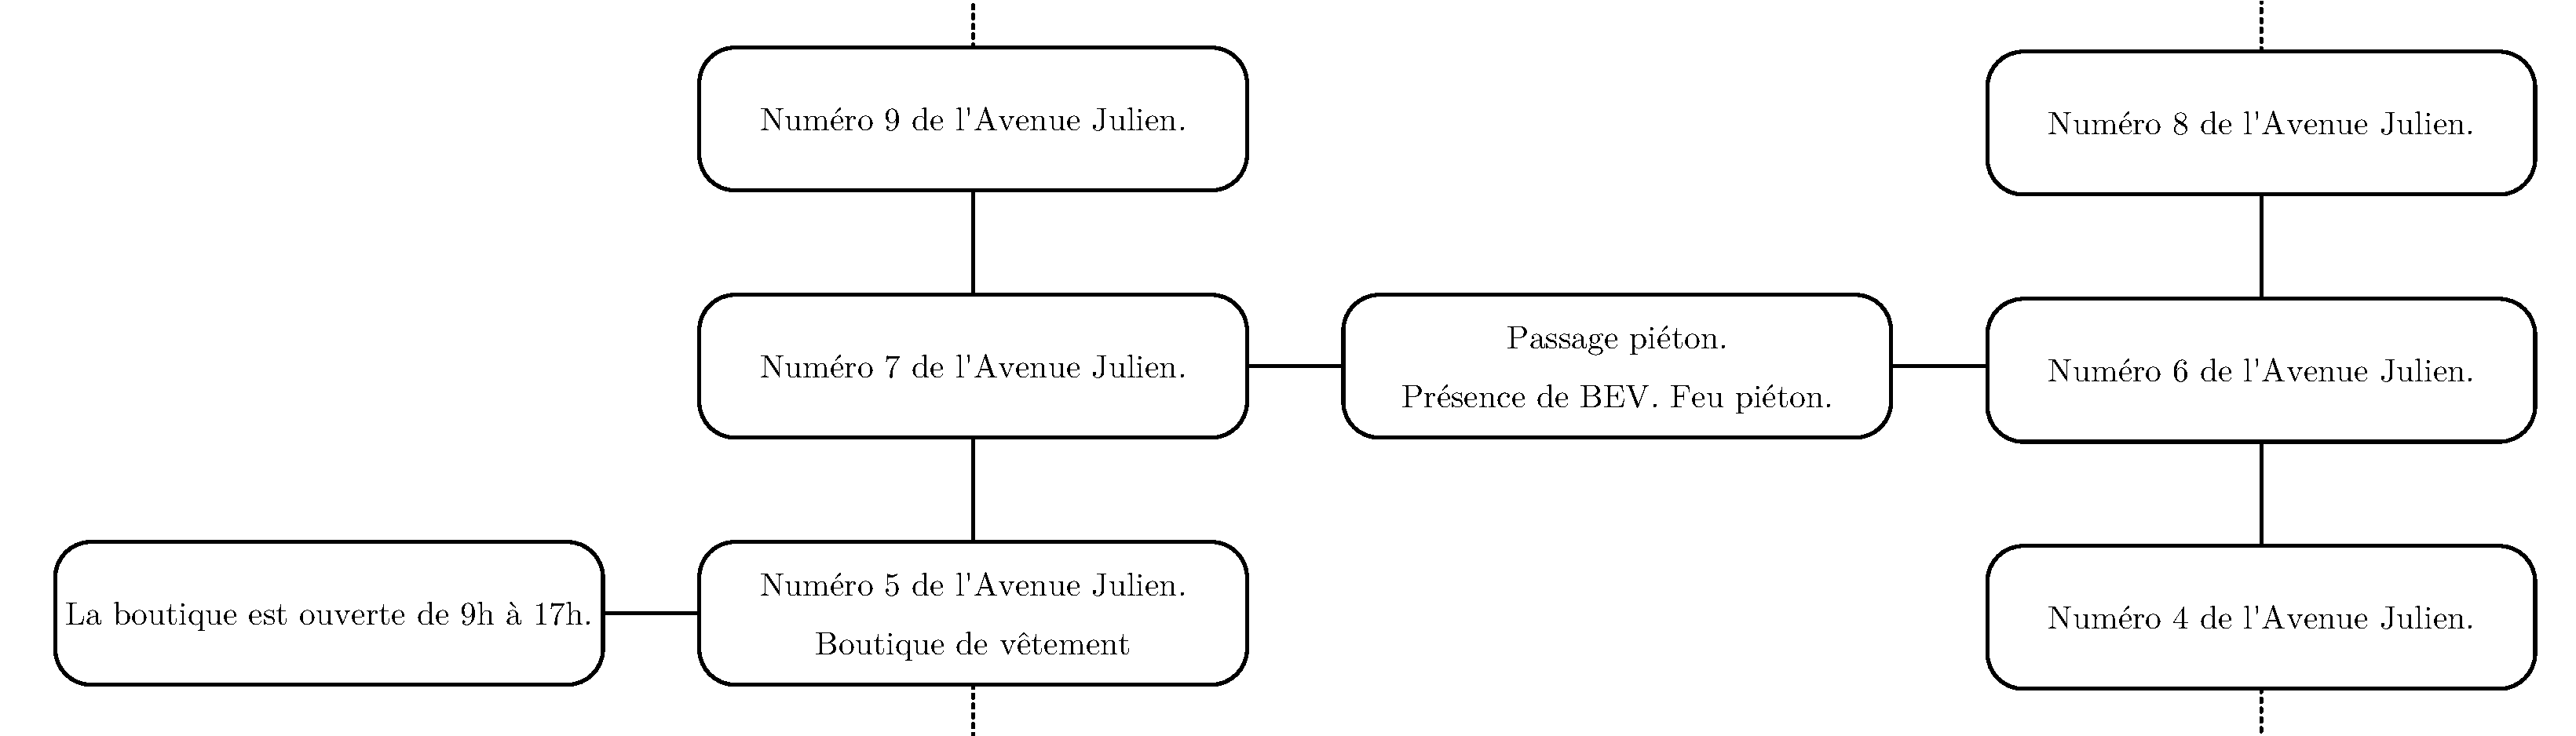
\includegraphics{images/description/exemple_desc_graphe.pdf}}
    \caption[Graphe de texte d'un tronçon de rue]{Un graphe de texte permet de représenter un environnement topologique, ici un tronçon de rue. Plusieurs nœuds peuvent dériver d'une même entité géographique (ici une boutique dont les horaires sont indiqués sur un nœud voisin).}
    \label{fig:desc_graphe_texte}
\end{figure}

\section{Conclusion du chapitre}

Dans ce chapitre, nous avons étudié la problématique de la description textuelle de données géographique, au-delà des carrefours, avec un focus particulier sur l'accessibilité du texte aux \gls{pcdv} à travers la hiérarchisation du texte. 

\newpar{}

Nous avons proposé un cadre de conception de description intégré à un \gls{sig}. Ce cadre propose de partir du besoin exprimé par l'\gls{ia} pour permettre à un géomaticien d'implémenter une chaîne de traitement qui, à partir de données géographiques, réalise la description nécessaire et permet d'appliquer, en fonction de la qualité des données, cette description sur plusieurs territoires. Le besoin de modularité exprimé par les instructeurs peut être intégré sous la forme de paramètres exposés par les chaînes de traitement permettant à l'exécution d'agir sur la description générée: verbosité, vocabulaire, etc. 

\newpar{}

Les outils permettant de réaliser la chaîne de traitement ont été implémentés dans le \gls{sig} QGIS et leur fonctionnement technique est présenté au chapitre \ref{chap:implementation}. Cette partie s'intéressera particulièrement à la réalisation de descriptions de carrefours en utilisant les outils présentés précédemment. Par ailleurs, l'évaluation des capacités du dispositif à générer des descriptions effectivement exprimées par des \gls{ia} est présentée en chapitre \ref{chap:evaluation}.